%You can delete all the comments after you have finished your document
%this sets up the defaults for the documents, 12pt font and A4 size. The article type sets this up as such as opposed to letter or memo.

%for the finer points LaTeX see https://en.wikibooks.org/wiki/LaTeX or http://tex.stackexchange.com/

\documentclass[12pt,a4paper]{article}
\usepackage{titlesec} %these are how we import packages, one helps set up footers and title layout
\usepackage{fancyhdr}

% !TEX TS-program = pdflatex
% !TEX encoding = UTF-8 Unicode
\usepackage[utf8]{inputenc} % set input encoding (not needed with XeLaTeX)

\usepackage{graphicx} % support the \includegraphics command and options
\graphicspath{ {./Images/}}

% \usepackage[parfill]{parskip} % Activate to begin paragraphs with an empty line rather than an indent

%%% PACKAGES
\usepackage{booktabs} % for much better looking tables
\usepackage{array} % for better arrays (eg matrices) in maths
\usepackage{paralist} % very flexible & customisable lists (eg. enumerate/itemize, etc.)
\usepackage{verbatim} % adds environment for commenting out blocks of text & for better verbatim
\usepackage{subfig} % make it possible to include more than one captioned figure/table in a single float
\usepackage[toc,page]{appendix}
\usepackage{titlesec}
% These packages are all incorporated in the memoir class to one degree or another...
\setcounter{secnumdepth}{4}

%header and footer settings
\pagestyle{fancyplain}
\fancyhf{}
\renewcommand{\headrulewidth}{0.5pt}
\renewcommand{\footrulewidth}{0.5pt}
\setlength{\headheight}{15pt}
\fancyhead[L]{Jonathan Mitchell - 40311730}
\fancyhead[R]{ SOC10101 Honours Project}
\fancyfoot[L]{}
\fancyfoot[C]{\thepage}

%set better section layout
\makeatletter
\renewcommand\subsection{\@startsection {subsection}{1}{2mm} % name, level, indent
	{3pt plus 2pt minus 1pt} % before skip
	{3pt plus 0pt} % after skip
	{\normalfont\bfseries}}
\makeatother
\makeatletter
\renewcommand\section{\@startsection {section}{1}{0mm} % name, level, indent
	{4pt plus 2pt minus 1pt} % before skip
	{4pt plus 0pt} % after skip
	{\bfseries}}
\makeatother

%this starts the document
\begin{document}
	
	%you can import other documents into your main one, these layout the Title and Declarations on its own page.
	%you might need to change these to \ if your on Microsoft Windows.
	\newcommand{\HRule}{\rule{\linewidth}{0.5mm}}

\begin{titlepage}
	\begin{center}

	\HRule \\[0.4cm]
    	{\Large \bfseries Exploring the Microservice Architecture to develop a flexible web-service of some description \par}
	\vspace{0.2cm}
	\HRule \\[1.5cm]

	
    	\vspace{3cm}
	\begin{minipage}{0.4\textwidth}
	\begin{center} \large
        \emph{}\\
        	Jonathan James Mitchell - 40311730
				
   	 \end{center}
    	\end{minipage}
	
	\vspace{2cm}
    	\begin{minipage}{1\textwidth}
    	\begin{center} \large
        
		Submitted in partial fulfilment of \\
		the requirements of Edinburgh Napier University \\
		for the Degree of \\
        	BEng (Hons) Software Engineering
    	\end{center}
    	\end{minipage}

    	\vfill

    	% Bottom of the page
	\begin{minipage}{1\textwidth}
    	\begin{center} \large
		School of Computing
    	\end{center}
    	\end{minipage}
	
	\vspace{1cm}
    	{\large \today}


	\end{center}
\end{titlepage}
%{\large Submitted in partial fulfilment of the requirements of Edinburgh Napier University for the Degree of }
	
\section*{Authorship Declaration}
\vspace{0.5cm}
\begin{flushleft}
I, Jonathan James Mitchell, confirm that this dissertation and the work presented in it are my own achievement.\newline

Where I have consulted the published work of others this is always clearly attributed;\newline

Where I have quoted from the work of others the source is always given. With the exception of such quotations this dissertation is entirely my own work;\newline

I have acknowledged all main sources of help; \newline

If my research follows on from previous work or is part of a larger collaborative research project I have made clear exactly what was done by others and what I have contributed myself;\newline

I have read and understand the penalties associated with Academic Misconduct.\newline

I also confirm that I have obtained informed consent from all people I have involved in the work in this dissertation following the School's ethical guidelines.\newline
\end{flushleft}

\begin{flushleft} \large
\emph{Signed: J.Mitchell} \\
\end{flushleft}

\vspace{.5cm}

\begin{flushleft} \large
\emph{Date: \today} \\
\end{flushleft}

\vspace{.5cm}

\begin{flushleft} \large
\emph{Matriculation no: 40311730}  \\
\end{flushleft}
	\pagebreak
	\section*{Data Protection Declaration}
\vspace{0.5cm}
\begin{flushleft}
Under the 1998 Data Protection Act, The University cannot disclose your grade to an unauthorised person. However, other students benefit from studying dissertations that have their grades attached. \newline

\vspace{0.5cm}

Please sign your name below one of the options below to state your preference.\newline
\vspace{0.5cm}

The University may make this dissertation, with indicative grade, available to others.\newline
\vspace{3cm}


The University may make this dissertation available to others, but the grade may not be disclosed.\newline
\vspace{3cm}


The University may not make this dissertation available to others.\newline
\end{flushleft}


	\pagebreak
	
	%LaTeX let you define the abstract separately so it wont get sucked into the main document.
	\begin{abstract}
		%Type stuff here
		This project is designed to explore the Microservice Architecture (MSA) to develop a flexible E-commerce web system. The architecture will be explored by researching and discussing various principles, tenets, architectures and technologies that can be used to develop web systems using MSA. Due to the architecture being relatively new; only being discussed and implemented in the last few years. There is no official consensus on how this architecture can be implemented. There are several suggestions and ideas available that are discussed and explored by members of the profession. These include suggestions such as: incorporating current principles like single-responsibility principle, that is part of the SOLID principle. Enforcing Domain Driven Design (DDD) to create bounded context for microservices to operate within and define where communication between microservices may be needed, automated testing and deployment pipelines and DevOps. 
		
		Modern technologies such as containerisation (Docker and Kubernetes) and the Cloud (Azure and Amazon Web Services(AWS)) are being suggested for use with MSA. These forms of Virtualisation aid in promoting a distributed system design - suggested for MSA. Using the Cloud for deployment purposes has contributed to the development of web-based systems. Integrated Development Environments (IDE's) such as Visual Studio, Eclipse and IntelliJ are available for this. 
		
	\end{abstract}
	\pagebreak
	
	\tableofcontents % is generated for you
	\newpage
	
	\listoftables
	%generated in same way as figures
	\newpage
	
	\listoffigures
	%you may have captions such as equations, listings etc they should all appear as required
	%these are done for you as long as you use \begin{figure}[placement settings] .. bla bla ... \end{figure}
	\newpage
	
	\section*{Acknowledgements}
	Insert acknowledgements here
	I would like to thank my supervisor, Xiaodong, for his advice and support with my dissertation. My Degus. My parents, Maya and Graham for listening to my rambling about my dissertation and attempts to explain it to them.
	\newpage
	\section{Chapter 1: Introduction}
	\subsection{Background}
	Traditionally, software applications/systems are developed using the Monolithic Architecture – a unified model of the design of a software program \cite{MonolithMargaret}. They are designed to be self-contained: components of the program are interconnected and interdependent. 
	For this tightly coupled architecture to work, each component and dependent component’s must be present for the code to compiled or executed. If any component is missing, there is a high chance the program will not work correctly.
	The rapid increase of software systems has changed the shape of how businesses function in today’s world. As businesses have expanded and added new products/services, problems arose where the Monolithic code base would become difficult to maintain and any future changes could result in problems arising when implemented.
	For the past thirty years, the software industry has been moving every closer to a service-orientated approach \cite{SoADummies}. This evolution has resulted in a closer bond between businesses and IT. Instead of businesses making decisions controlled or constrained by software, they now make decision supported by software. 
	
	Service Orientated Architectures (SOA) were the first realisation of transforming monolithic systems into small building blocks – components – that work together to create applications that are easier to maintain and expand upon. A service is defined as: a function that is well-defined, self-contained, and does not depend on the context or state of other services \cite{ServiceArchiBarry}.
	Around seven years ago, at a workshop of architects in Venice, the participants saw a common architectural style they had all been recently exploring. The term “Microservices” was created \cite{MartinFowlersite}. It describes a particular way of designing software applications as suites of independently deployable services. That can be maintained and modified effectively to meet the demands of the business world in the present day.
	
	By describing each function, of a software system, as an individual service; they can be separated into their own components, contained within their own domain model. Doing this entails each service has a single responsibility to perform and no more. This would also entail each service to have its own database with which to manipulate data. There would be no shared relational database for the entire system. Although there may be a need for different services to communicate with each if they share specific information in order to maintain the validity of data their databases. The development of containerised software has increased the capability of polyglot programming. Were each Microservice can be written in a different language, and when deployed via containers, they combine, like building blocks, to form the software system. This form of modularity allows for each Microservice to function independently and improves the stability of the system as a whole - if one Microservice was to fail, it would not result in the entire system from failing. 
	
	With the recent boom of the internet, particularly in the last decade, Microservices are beginning to be used by retail companies with a large online presence such as: Amazon, Netflix and Ebay. Although retail is not the only sector to use this architecture: Uber, the guardian and Capital One. As the internet has proven to be an excellent platform to deploy systems. More specifically web-based systems.
	
	This project investigates and evaluates: designs, principles and technologies related to Microservices used too implement this architecture in developing an E-Commerce web system.
	\subsection{Motivation}
	why are you doing this? needed?
	
	\subsection{Aims, Objectives and Scope}
	The aim of this project is to explore how a Microservice architecture (MSA) can be used to develop a flexible web based E-commerce system. Finding out the flexibility such an architecture provides and how this can be used to allow developers too maintain/update such systems in the fast-paced environment of today’s world. This project will concentrate on developing a web-based system as the internet has been one of the fastest growing resources available to businesses to expand and meet the ever growing demands of customers. 
	 
	These aims are achieved by examining the literature available on Microservices, the principles involved to enforce the Microservice Architecture and the technologies available to create this architecture for developing software to define research questions.
	A software development environment is then chosen to implement this architecture in a prototype system.
	Literature research will include: academic white papers, professional journals, lectures, on-line articles and software books. The collected/researched information will be used to answer the questions and provide the necessary understanding to develop a prototype using the Microservice architecture. Following this, the project is evaluated, considering the original aims and objectives.
	
	As MSA is a relatively new architecture; there is still a broad view for successful implementation. Due to time and cost constraints, this project will focus on web-based design patterns and protocols. As well as software and hardware to design a web system. There will be a limit to the exploration of  applicable principles, design patterns, hardware and software available that cna be used to implement a Microservice architecture.
	
	\subsection{Outline}
	This dissertation is structured as follows:
		\begin{itemize}\itemsep0pt
			\item \textbf{Chapter 1: Introduction}
			\\Introduces the topic of Microservices, names the aims and objectives and outlines the scope and constraints for this project.
			\item \textbf{Chapter 2: Literature Review}
			\\Encompasses all the subjects and terms that are related/representative of a microservice architecture. It will go into detail about why Microservices are being used, why it is preferred over Service-orientated architecture and the technologies currently in use and those being developed. This chapter will also provide a critical and objective analysis of these subjects. 
			\item \textbf{Chapter 3: Project Planning}
			\\Provides an overview of the management of the project. With use of a Gantt chart. The methodologies used during the development cycle will also be described. With justification. This chapter will also include a description of the high level functionality needed for the project using the project management tool MoSCoW.
			\item \textbf{Chapter 4: Prototype} 
			\\ This chapter contains the following sections:
				\begin{itemize}
					\item \textbf{Analysis}
					\\This chapter will describe the requirements for the development of a prototype. And an analysis of the high-level design of the prototype. Including a diagram of the service interaction.
					\item \textbf{Design}
					\\This chapter will provide a detailed design of the structure of the prototype – UI designs, Class diagrams, E-R models etc.
					\item \textbf{Implementation}
					\\This chapter will detail the actual development of the prototype. Each staged will be documented. All issues/problems will also be documented along with the solutions. Also, providing a reference for all sources used. Screen shots of the development stages will be provided via appendices.
					\item \textbf{Testing}
					\\This chapter will consist of all testing documentation and testing conducted on the prototype. With a description of the testing methodologies used.
					\item \textbf{Evaluation}
					\\This chapter will provide a critical and objective analysis of the developed prototype. Providing a detailed description of its success/failure.
				\end{itemize}
			\item Chapter 5: Conclusions
			\\Discusses the project, how effective Microservices architecture is etc. And going forward what further research etc. will be done/required.
			\item Chapter 6: References
			\\Contains all references used throughout this document.
			\item Chapter 7: Appendices
			\\Houses all the appendices. This includes Gantt charts, UML diagrams, testing documentation and screen shots of: development progress at various stages and working prototype.
		\end{itemize}
	\subsection{Summary}
	This project will review the following principles, design patterns and technology:
	\begin{itemize}
		\item Single Responsibility Principle
		\item Model-View-Controller (MVC) Architecture
		\item RESTful Architecture
		\item Domain Driven Design (DDD)
		\item Docker for Containerisation
		\item Kubernetes??
		\item Visual Studio using ASP.net
		\item IntelliJ web development
	\end{itemize}
	Being a prototype, and a university project, the system will not implement a payment system nor will the login/authentication Microservice require any more than a login and password. No personal details will be requested. Nor will any anonymous logging fo user interaction be logged/recorded.
	\pagebreak
	\section{Chapter 2: Literary Review}
	\subsection{Microservice}
	This chapter discusses the Microservice architecture. It also discusses why this architecture is being preferred over the service-orientated architecture.

The term “Microservice” was first used at a software architects workshop held in Venice in May 2011 as stated by Martin Fowler \cite{MartinFowlersite}. Participants began to realise they were using and exploring the same architectural style. It was a year later it was decided as the more appropriate name \cite{MartinFowlersite}.
As Microservices Architecture (MSA) is a relatively new architecture, there is no official industry consensus regarding the properties nor definition of MSA.

According to Sam Newman \cite{NewmanMSA} Microservices are: “small, autonomous services that work together”. Martin Fowler \cite{MartinFowlersite} continues this definition by saying “Microservices are a way of designing software applications as suites of independently deployable services”.
Microservices help break the boundaries of large applications and create smaller systems (the services) that are used to build applications as seen in figure \ref{fig:MonovMSA}.
\begin{figure}[h]
	\caption{Monolithic vs Microservices Architecture}
	\label{fig:MonovMSA}
	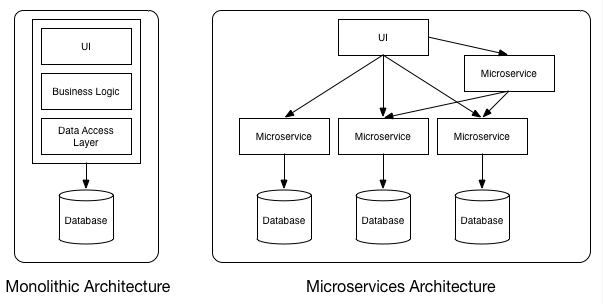
\includegraphics{MSAexample}
	\centering
\end{figure}
Tomas Cerny et al \cite{ContextUnderstandingMSA} have described Microservices as being based on three Unix ideas:
\begin{itemize}
	\item A program should fulfil only one task and do it well
	\item Programs should be able to work together
	\item Programs should use a universal interface
\end{itemize}
The implementation of MSA is open to interpretation. Though there are some defining characteristics that are commonly cited \cite{GuptaMSA} \cite{MartinFowlersite} \cite{ContextUnderstandingMSA}. Although
Zimmerman in his paper \cite{Zimmermann2017} explores the argument that the Microservice architecture itself is in fact not an Architecture but an implementation of the Service Orientated Architecture. But does state there is, currently, no consensus on the relationship between MSA and SOA.

\subsubsection{Services Are independently deployable}
Unlike traditional monolithic applications that contain several modules that may be dependent on several libraries, environment etc. Each service, within a Microservice architecture, can be deployed independently. All dependencies: database, library dependencies and execution environments such as web servers or Virtual Machine (VM) are contained within each service. This ability is what enables each service to deploy independently and be essentially autonomous as described by Gupta \cite{GuptaMSA}. Therefore, each individual service will only contain the dependencies it needs. And can be deployed for use and perform its intended function. Even if no other service is available, the deployed services will perform their intended function, barring failure: hardware, software etc.

As services can be deployed on different machines, a distributed system of services, this can help with fault tolerance. If only a single service is on a machine that fails for whatever reason. Then it will not affect the rest of the services increasing the fault tolerance of the system or program.

Each of the independent services deployed combine to make the intended application(s). Such as an E-Commerce web application, news web application etc.

\subsubsection{Services are built around business capabilities}
The more recognised model of focusing on the technology layer of applications results in creating different development teams for: UI, server-logic, database etc. Having such separated teams separated like this, simple changes to any aspect can result in delays of development due to cross-team communication, budgets etc. This results in an application created that follows Conway’s law \cite{ConwayLaw}: “Any organization that designs a system (defined broadly) will produce a design whose structure is a copy of the organization's communication structure.” See figure \ref{fig:CowayLaw}.
\begin{figure}[h]
	\caption{Conway's Law}
	\label{fig:CowayLaw}
	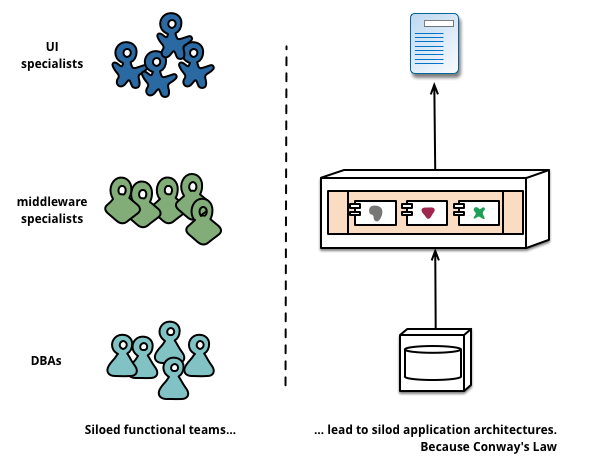
\includegraphics{ConwaysLaw}
	\centering
\end{figure}
The Microservice approach changes the view of division with development teams. This approach involves organising teams around developing services based on the businesses capabilities – accounts service, basket service, payment service, catalogue service, car insurance service etc. These services implement the software needed for that business area: UI, storage, external collaborations etc. The teams become cross-functional consequently, including the full range of skills required for development: database, project management, UI etc. As described by Martin Fowler \cite{MartinFowlersite} in figure \ref{fig:busCapa}. 
\begin{figure}[h]
	\caption{Built around Business Capabilities}
	\label{fig:busCapa}
	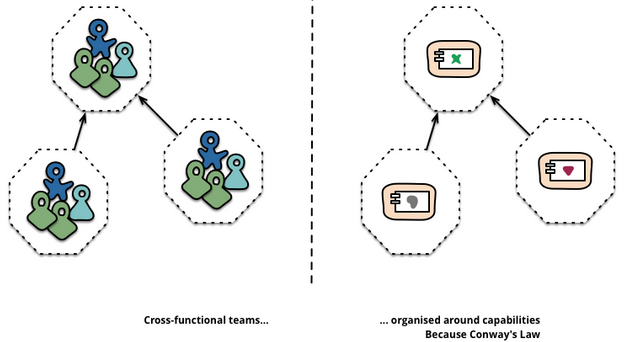
\includegraphics{ConwaysLawOpposite}
	\centering
\end{figure}

\subsubsection{Services are fine-grained Interfaces}
Small, performing only one function – each service is designed to have only one responsibility, perform a single functionality of the business. This single responsibility principle also encompasses the database in use. Instead of having a single database used in a monolithic system, each Microservice can have its own database to store the data. This is a change from the Monolithic style where a single database would be used to store the systems data. Although, several Microservice could access the same database, again, depending on the context of the software system.

The services are described as “fine grained” referring to the granularity of the Services themselves. The actual size of the service varies depending on the context of the business. How small or fine grained a service must be is open for discussion. A general agreement is that the codebase of the service should be manageable by a small team of people.  For example, Amazon \cite{HoffAmazonArchi} has coined the phrase “the two-pizza teams” – each team numbers around 8-10 people. The number you can feed off two pizzas . Meaning the code base for the Microservice would only be “big enough” for this number of people to handle. Similarly, Jon Eaves, of RealEstate.com.au, characterizes a Microservice as something that could be rewritten in two weeks as stated by Sam Newman \cite{NewmanMSA}).

Zimmerman \cite{Zimmermann2017} reinforces this definition of: "Services that can be deployed,c hanged, substituted and scaled independently of each other" and states fine-grained services as one of the seven common tenets cited in introductory literature and case studies on Microservices.

\subsubsection{Services are designed to fail}
By creating services as components, applications that use these services need to be designed so they tolerate any failure of services \cite{MartinFowlersite}. This introduces another layer of complexity when designing microservices. Services can and will fail, but the effect on users must be limited.

It is important to detect failures as quickly as possible and restore them, automatically if possible. The MSA puts emphasis on real-time monitoring of the application; checking architectural (database requests per second) and business relevant (orders per minute received etc) metrics \cite{MartinFowlersite}. Monitoring can lead to early warning signs of a failure, that will allow development teams to proactively investigate.

This will likely lead to complex, and expensive, monitoring systems in place – The Microservice teams need to know which services, running in different processes, have failed. This is generally achieved by having separate, sophisticated monitors and logging set-ups for each service available. Monitoring such things as: up/down status and operational/business relevant metrics \cite{MartinFowlersite}.

Famously, Netflix created a set of tools dubbed the “Simian army” that were developed solely to generate various kinds of failures and test the robustness of their system. \cite{SimianArmy}. 

\subsubsection{Microservice Architecture has a natural modular Structure}
As described previously, each service is a component of the system and, thus, enforces a modular structure where each service is seen as a module. This implementation of Modular Programming \cite{TechopediaModular} encompasses many of its benefits:

Each service can be used many times by many users. This benefit is adhered too as the code written, for each service, is not repeated. Only the service needed is called upon, through events etc., and executes the required task(s).

This modularity allows for each service to be used in conjunction with other applications. As service independence is a requirement of the MSA, the services can be used in the creation of multiple applications.

A disadvantage with the modular structure of the Microservice architecture occurs in the debugging of the system.  

\subsubsection{Encourages Infrastructure Automation and Testing}
As different businesses have different needs, the number of microservices developed can differ greatly. As the Microservice architecture adheres to the distributed systems model; microservices will be deployable on multiple servers/machines and it can become difficult, almost impossible, to develop, test, deploy, monitor each Microservice manually. Regardless of the size \& number of software development teams. The answer to this is to introduce automation. 

The development of the Cloud and Amazon Web Services (AWS) have reduced the operational complexity of building, deploying and operating microservices \cite{MartinFowlersite}. These infrastructure automation techniques have evolved extensively over the last few years.

Current systems built using microservices are development by teams with extensive Continuous delivery (discussed later) experience \cite{MartinFowlersite}. Software built using this principle make extensive use of the above infrastructure automation techniques. This helps to streamline and automate the testing of builds.  See figure \ref{fig:autoTestDeploy}.
\begin{figure}[h]
	\caption{Automated testing to deployment}
	\label{fig:autoTestDeploy}
	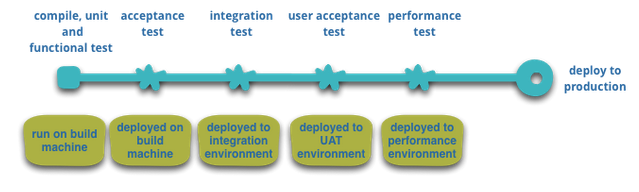
\includegraphics{AutomatedTestingDeployment}
	\centering
\end{figure}
Current systems built using microservices are development by teams with extensive Continuous delivery (discussed later) experience (Fowler, 2014). Software built using this principle make extensive use of the above infrastructure automation techniques. This helps to streamline and automate the testing of builds.

Testing and deployment automation brings several advantages:
\begin{itemize}
	\item allows teams to choose when they want to deploy the microservices they are in control of. Potentially deploying new builds multiple times in a short period of time.
	\item Newly developed/updated features are in the hands of customers faster
	\item Allows for frequent testing of new features
	\item Teams can experiment new processes, algorithms etc. Lokesh Gupta \cite{GuptaMSA} describes this as Enterprises being given the ability to experiment and fail fast.
\end{itemize}
But there are disadvantages.
A potential risk to continuous deployment/integration is “moving fast and breaking things” \cite{HunterAdvMSA}. If backward compatibility is not diligently adhered too, for versioning deployments, a change can be released that results in the Microservice breaking and affecting consumers.
\subsubsection{Introduces the concept of you built it you own it}
Depending on the scale of the services provided by companies, there can be hundreds of microservices within a company’s software system structure. For example, Amazon, one of the first companies to embrace MSA, has over 150 services and can up to 100 of these services to build a single web page \cite{HoffAmazonArchi}. Services include: Search, register, account, catalogue, refine, recommendations etc.

	
	\pagebreak
	\subsection{Domain Driven Design}
	This section covers Domain Driven Design. Software development is made complex by multiple factors. One of these being the problem domain. 
\subsubsection{The Domain}
Eric Evans \cite{EvansDDD} describes the domain, of any software program, as the representation of a real-world domain. Such as an airline booking program booking people onto an air plane, a finance software system dealing with money and finance. He goes on to explain that the domain is formed from models that are a simplification of aspects of a real-world domain.

\subsubsection{Bounded Context}
The bounded context of Domain Driven Design is described as the boundary of a coherent part of the business by Andreas et al \cite{mci/Diepenbrock2017}. Martin Fowler \cite{MFowlerDDD} provides a similar description when he says that the bounded context is necessary when creating a software system based on a large business domain. As it is difficult to build a single, unified model. Eric Evans \cite{EvansDDD} has a similar view point to this.
Each bounded Context defines what is to be included within it, what is not and its relationship with other bounded contexts, this includes communication. Each bounded context, in a software system, contains a model that is a representation of a real world aspect of the business domain. The model would contain classes, attributes and methods that describe domain concepts. Martin Fowler explains: "To be effective, a model needs to be unified - that is to be internally consistent so that there are no contradictions within it." \cite{MFowlerDDD}
For example (should I include this?), In the context of this project. A bounded context for the software system could be a customer support/services Context. The Context-model of this business Domain could contain the following classes:
\begin{itemize}
	\item Customer 
	\\ Contains the attributes that represents a customer - name, contact details etc. 
	\item Ticket
	\\ Attributes including ticket number, type of issue, description, order number related to it etc.
	\item Ticket communication
	\\ Contains information on what has been done to resolve the issue 
	\item Product
	\\ Provides a description of the product - name, type, price etc.
\end{itemize}
From this example, it can be deduced that other bounded contexts will be created, to model the other aspects of the business domain and these contexts would then combine to model the actual business domain itself. Some of the bounded contexts modelling will contain similar classes, with similar attributes. Such as the above Customer and Product Classes. These would be similar to, for example, a context of the sales context. This model would contain a class for customer and product. The former being the customers identity and the latter the description of the product. There would be some form of communication between these contexts to ensure the data help in each model is the same, were shared. So both contexts are consistent within themselves and as models of the domain.

As each Bounded Context is conceptualised, the individual Microservices can be discovered. There are issues with using this design for discovering Microservices. Florian Rademacher et al\cite{DDDChallenges} discuses how using Domain Driven Design omits the following information when deducing the Microservices and their characteristics:
\begin{itemize}
	\item Interfaces and operations
	\item operational parameters and return types
	\item endpoints, protocols and message formats
\end{itemize}
	\pagebreak
	\subsection{Single-Responsibility Principle}
	 Single Responsibility Principle (SRP) is one of the SOLID Principles described by Robert Martin \cite{RobMartCleanArchi}.
 He proposes this principle follows on from Conway's Law: the structure of a software system mirrors the communication design of the business that uses the software and that each module should only have one reason to change. And each software module should only be responsible for a single actor, not do just one thing.
 Each Microservice should be its own module, within MSA, and have a single responsibility to provides its intended service a single actor - be that for a user, stakeholder, internal software process, business policy etc. This design principle ensures each microservices is easy to understand and maintainable: allowing for changes to occur based on the requirements of the users. 
 Another benefit provided is each service can be used as the basis of components to be used in many different software systems. Creating the notion that services themselves are modular in design.
 Using this principle in developing microservices enforces cohesiveness. Each class, function etc of a Microservice combine to form the Microservice. 
 Microservices take the single responsibility a step further by also including the data storage (database) as part of the principle. Monolithic software systems share a single, large database for data storage. The Microservice Architecture is designed so each Microservice has its own database, purely to store the data it needs. Nothing else.
 
 This addition to the SRP ensures there is very little, if any, coupling between Microservices. And prevents any actions from a Microservices affecting any other Microservice of the system.
	\pagebreak
	\subsection{RESTful}
	\input{Chapter2/RESTful}
	\pagebreak
	\subsection{Polyglotism}
	\subsubsection{Polyglot Programming}
Believe to be first introduced in 2006 by Neal Ford \cite{PolyglotOrigins}.
Polyglot programming is the practice of writing code, for applications, in multiple languages \cite{PolyglotProgTechTarget} as applications are becoming more complex, in design and functionality, different types of problems occur. This is done to add functionality, efficiency and to tackle specific problems \cite{PolyglotMFowler}, to applications, when a single language can't provide everything required. 

For example, building an E-commerce website would likely involve developing the system using: C\#/Java, Python, JavaScript and HTML5. The document formatting language (CSS) and data query language (SQL) could also be used. JavaScript, HTML5 \& CSS would also be used for user Interface design. C\# and/or Java can be used for Object-orientated functionality etc. SQL would be used for database manipulation/interrogation. Python could be used to provide security protection for applications.

The microservice architecture, being a distributed system, can incorporate polyglot programming extensively. Besides the above mentioned, various microservices could be written in different programming languages, to take advantage of functionality only present in them. 

However, including Polyglot Programming into an application is likely to add complexity to the system. Developers will need to learn the range of languages present or teams will need developers proficient in the required languages.
\subsubsection{Polyglot Persistence}
Believed to have been first conceived by Scott Leberknight \cite{PolyglotPersistLeberknight}. Polyglot Persistence is the practice of having various database technologies to store persistent data. With the introduction of NoSQL Databases, and other non-traditional data stores, the move away from using only a Relational Database Management System (RDBMS) to store data began. 

Similar to polyglot programming, the increased complexity of applications also incurs problems when it comes to storing data. As the variety of data to be stored increases, such as big data, the traditional structured RDBMS is not always suitable. Applications may need data to be stored regularly, if there is multiple users using its services at any one time.

NoSQL databases allows for a variety of unstructured data to be store successfully. Data, keeping in context of this project, such as a customer's basket would not be consistent in what it stores - each item in the basket will possibly have different information stored about it. Adding the fact multiple customers will be using an E-commerce web system at the same time, the velocity of data inserts will be potentially be fast and NoSQL Databases (DB's) can handle this well. They provide Horizontal and vertical scaling. Providing greater benefit than most RDBMS which are limited to vertical scaling
As seen in figure \ref{fig:PolyglotPersistence} \cite{PolyglotSerra}:
\begin{figure}[h]
	\caption{Polyglot Persistence Implementation example}
	\label{fig:PolyglotPersistence}
	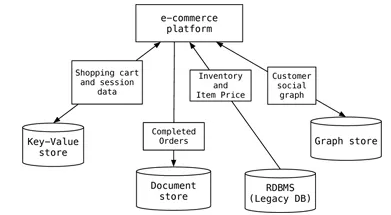
\includegraphics{PolyglotPersistence}
	\centering
\end{figure}

As with Polyglot Programming, Polyglot Persistence adds complexity as each data storage technology added involves learning how they work \cite{PolyglotSerra}.



	\pagebreak
	\subsection{Virtualisation}
	blah
	\pagebreak
	\subsection{Asp.Net}
	blah
		\subsubsection{Razor Pages}
		blah
	\pagebreak
		\subsection{Java Web Development}
	blah
	\pagebreak
	\subsection{Conclusion}
	In Summary, the literary review has provided material enough to describe the benefits associated with the Microservice Architecture and the disadvantages.

There is an argument the Microservice Architecture is an effective implementation of the Service-orientated Architecture. There is also evidence to support it is its own architecture aswell.

The separation of services into individual, distributed modules does have its benefits in terms of being able to administer maintenance: bug fixes, adding new function. Also the notion of each service representing a different business capability allowing for distributed teams: each working on a different microservice does allow for teams to ''own'' the microservices they work on. 

The benefit of polyglotism is apparent when using microservices. Individual teams specialising in different programming and database languages, allow for each Microservice to be developed in the language that fulfils its requirements the best. This also includes the accompanying database, if one is required. A downside to this is that only teams or individuals with the knowledge of language used can maintain it.

The use of docker or other container-based software like Kubernetes allows for any Microservice to be deployed from any machine that is able to run the underlying virtualisation software. Learning Docker can be a steep learning curve, even with IDE's providing automation of some of the features. There is significant underlying infrastructure needed for communication to microservices from the front-end interface.

As the microservice architecture is relatively new, there are different views on how the architecture design should be implemented. Some are still being researched and written about.

Of note is the different take on the use of databases. This project will develop a prototype with both styles of database available. Each will be tested individually for all available CRUD implementation for each Microservice. Recording the response times for each and presenting this data, in a visual form, to show which is faster and which style should be preferred for Microservice Architectures.

The following will be used to evaluate this project:
\begin{itemize}
	\item The proposed design of the system\\
	The proposed Design will involve the features and design patterns discussed previously. Involving class diagrams, Microservice interactions, domains etc.
	\item A successful prototype developed\\
	Developed based on the proposed design, with an evaluation including the difficulties and easiness in adhering to the design. With a discussion on the advantages/disadvantages of the design. Looking into potential improvements.
	\item An evaluation of both database styles: centralised and separate\\
	This will be conducted by simulating use of the website, using testing software described previously, and displaying the gathered data of when the different database styles are queried. Displaying response times and comparing them to help determine why the separated database design is chosen over a centralised one.
\end{itemize}
	\pagebreak
	\section{Chapter 3: Proposed Design}
	\subsection{Test}
	blah blah blah
	\pagebreak
	\section{Chapter 4: Prototype}
	\subsection{Analysis}
	\subsection{Requirement Specification}
	The following Requirement Specification was devised form the analysis:
	\subsubsection{Purpose}
The purpose of this document is too detail the requirements of the project's Web system Prototype. The Requirement specification contains the following headlines:
\begin{itemize}
	\item Project Brief - provides a description of the web system prototype. %as there is no "client" this may be the best option atm.
	\item Scope - details the size of the project
	\item Resources - What suitable resources have been sourced to implement the prototype 
	\item User Requirements - Provides a description of the services provided to users
	\item System Overview - contains an overview of what the system will do
	\item System Architecture - provides a high-level understanding of the design structure of the web system
	\item Functional Requirements - Details what each Microservices function
	\item Non-Functional Requirements - details the design of the front-end web User Interface (UI)
	\item Performance - contains the expected performance of the system
\end{itemize}
\subsubsection{Project Brief}
The prototype to be created will be an E-commerce web system. The web system will allow users to perform actions commonly associated with E-commerce web systems.

This prototype will provide basic functions commonly found in E-commerce websites:
\begin{itemize}
	\item A simple authentication service in the form of register and login
	\item Search for specific catalogue items
	\item Add items to Basket 
	\item manipulate items in the basket - edit/delete items
	\item Deal of the week
\end{itemize}
These functions will form the bounded context of Microservices within this prototype.

Due to this being a prototype system and the constraints of being a university student, in terms of confidentiality and data protection, this prototype will not be providing a means to buy items. And the register function will only ask for a user name and password to be created by the user. no personal data will be requested.
\subsubsection{Scope}
The web system will allow users to register a login name and password to use the features of the site. The catalogue available for browsing will be limited to a few items under the following categories:
\begin{itemize}
	\item clothes 
	\item toys  
	\item Electronics 
	\item books 
	\item miscellaneous
\end{itemize}
Users will also be able to add more than one item to their basket, selecting the quantity of each item they want to add.

The web system prototype must be usable for all major web browsers. The User Interface (UI) will be a simple and non-complex design so users can use it successfully.

This prototype will be finished by -Insert date xx/xx/2019- 
\subsubsection{Resources}
This project will use the following development software:
\begin{itemize}
	\item Microsoft Visual Studio - to develop the web system prototype using asp.net
	\item Programming code - C\# will be used to write the coding of the software and SQL will be used for all database query command
	\item Microsoft Visio - To create the UML diagrams used for the Analysis \& Design stages
	\item TeXstudio - Used to write up any documents required
	\item SQLite/Entity Framework - this will be used to store necessary data permanently
\end{itemize}
\subsubsection{User Requirement}

\subsubsection{System Overview}
The project will a web system that can run on the main web browsers available: Mozilla Firefox, Google Chrome, Microsoft Edge, Opera, Safari.

The Web system will provide several web pages that provide the user with different information and functionality depending on that web pages requirements.

Each Microservice will perform a single function that is derived from the business domain and bound within the context of that domain.

To simulate a distributed system, the web system and some microservices will be separated and treated as a client-server set up. Where by the Microservice(s) will be communicated with over the local host of the machine used for deployment.

Visual Studio will be used to develop the web system. 

The business model, databases, will be created using the Entity framework or SQLite. And each Microservice will have its own database that it is solely responsible.
\subsubsection{System Architecture}
The web system will incorporate the following architectures and design principles:
	\begin{itemize}\itemsep0pt
	\item \textbf{Microservice Architecture}
	\\This will be used for the high-level design of the website.
	\item \textbf{Model-View-Controller (MVC)}
	\\This layered Architecture style will be used within the front-end user Interface.This layered Architecture will also be the entry point to access the API gateway to access the required Microservice.
	\item \textbf{RESTful API}
	\\Used within the MVC architecture to provide the communication between the UI and Microservices in regards to database usage. Implementing GET,PUT,DELETE and POST HTTP methodologies.
	\item \textbf{API Gateway Pattern}
	\\Used to provide the access for the front-end User Interface to the individual Microservices available. The API gateway will provide the methods needed to access the required Microservice.
	\item \textbf{Domain Driven Design (DDD) Principle}
	\\ The model layer will be created using this principle so each model will be constructed to contain the business domain it was constructed for and each model will have its bounded context.
	\item \textbf{Single Responsibility Principle}
	\\ Will coincide with the above principle to be enforced and ensures each Microservice has only one main function to perform and, thusly, will only require minor changes for future expansion/maintenance
	\end{itemize}
\subsubsection{Functional Requirements}
The functional requirements will display the microservices to be developed and the functionality associated with each.
The web system will provide the following Microservices:
\begin{itemize}
	\item Authentication service
	\item Catalogue service
	\item Search Service
	\item Basket service
	\item payment service?
	\item Administrator Service
	\item Customer service service
	\item customer service
\end{itemize}
And provide the following functionality:
	\paragraph{Authentication Service}
		\begin{itemize}
			\item Provide users the ability to register
			\item Provide users the ability to login
			\item identify type of user logging in - customer or administrator
		\end{itemize}
	\paragraph{Catalogue Service}
		\begin{itemize}
			\item Fill the home page with a selection of available items
			\item Provide a detailed description of each item selected by a user
			\item Allow the user to select more than one of an item to buy
			\item Allow users to add items to their list
		\end{itemize}
	\paragraph{Search Service}
		\begin{itemize}
			\item Allow users to search for specific items from the catalogue
		\end{itemize}
	\paragraph{Basket Service}
		\begin{itemize}
			\item Allow users to view the items in their "basket"
			\item Allow users to edit their basket - delete items and increase/decrease the number ordered of individual items
		\end{itemize}
	\paragraph{Payment Service}
		\begin{itemize}
			\item Allows users to view their items they wish to buy
			\item Provide Users with options on how they want items delivered
			\item Provide Users with multiple Payment options
			\item Display an invoice of the order made
			\item send an email confirmation of the order to the customer
		\end{itemize}
	\paragraph{Administrator service}
	\paragraph{Customer service service}
	\paragraph{Customer service}
		\begin{itemize}
			\item Provide Customers the ability to view previous orders
			\item Provide Customers the ability to view lists they have created
			\item Allow uses to change their password if needed
		\end{itemize}
\subsubsection{Non-Functional Requirements}
\subsubsection{Performance}
\subsubsection{Glossary}

	\subsection{Design}
	\pagebreak
	\subsection{Development}
	\subsubsection{Prototype Development with separate databases}
Developing the prototype began with creating the Catalogue Microservice first. This appeared to be a good place to start: create a basic MVC (Model-View-Controller) front-end that would connect to the Catalogue Microservice to display the list of items in the catalogue. Initially the idea was to create the Databases, with a table with data, connect to the microservice and then, through the API Gateway, connect with the front-end. Through research, it was deemed this was a difficult task to do. 

The API Gateway itself being a implemented using JSON documents and using a middle-ware technology, such as Ocelot Insert Citation, to implement. This would need further researching purely for this section of the prototype.

Instead, creating a blank Database was decided upon. From here, connect it to the API for the microservice and then to the front-end. The API Gateway has been omitted, at this stage, purely as there is only one API and to see the system working, albeit in a very basic way. Future, successful additions of microservices will see the API Gateway being added. 

NOTE: Docker support was added to begin with, but proved to be difficult to work with. Instead, the prototype was developed without Docker support. Which will be added later, after further researching and small prototype builds to use the features needed for this project. This decision was taken as it was necessary to provide a working prototype of the proposed system within the time-frame than being delayed by understanding and then fixing the problem incurred using Docker. If docker is not able to be added to the prototype. Then this will be documented in the evaluation section and discussed as fully as possible.

\subsubsection{Catalogue Microservice}
Creating the database was relatively simple: creating an account with Azure and creating the database and the server for its use. From here, the connection information needed is provided by Azure. Conveniently providing string connections depending on the type of connection wanted. ADO.NET was chosen. All that would be needed is having the string connection copy and pasted into the Appsettings.JSON file of the Catalogue Microservice. By adding the string to this file, enables Visual Studio to locate and connect to the server successfully to begin Entity Framework coding for manipulation/interrogation of the database.
\begin{figure}[h]
	\caption{Azure ADO.NET Connection String for the server containing the Catalogue Microservice Database}
	\label{fig:AzureCataMSImage}
	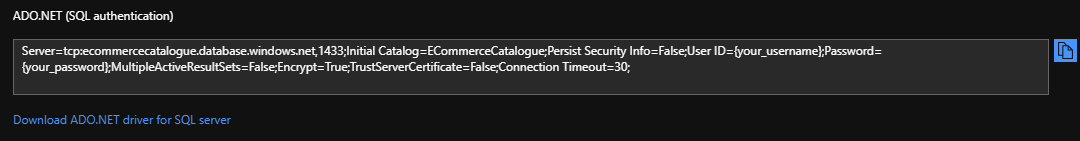
\includegraphics[height=3cm, width=20cm]{/DevelopmentPics/AzureCatalogueMSImage}
\end{figure}
\pagebreak
\begin{figure}[h]
	\caption{Visual Studio Appsetting.JSON connection string. Partial View}
	\label{fig:VSPartialCataMSImage}
	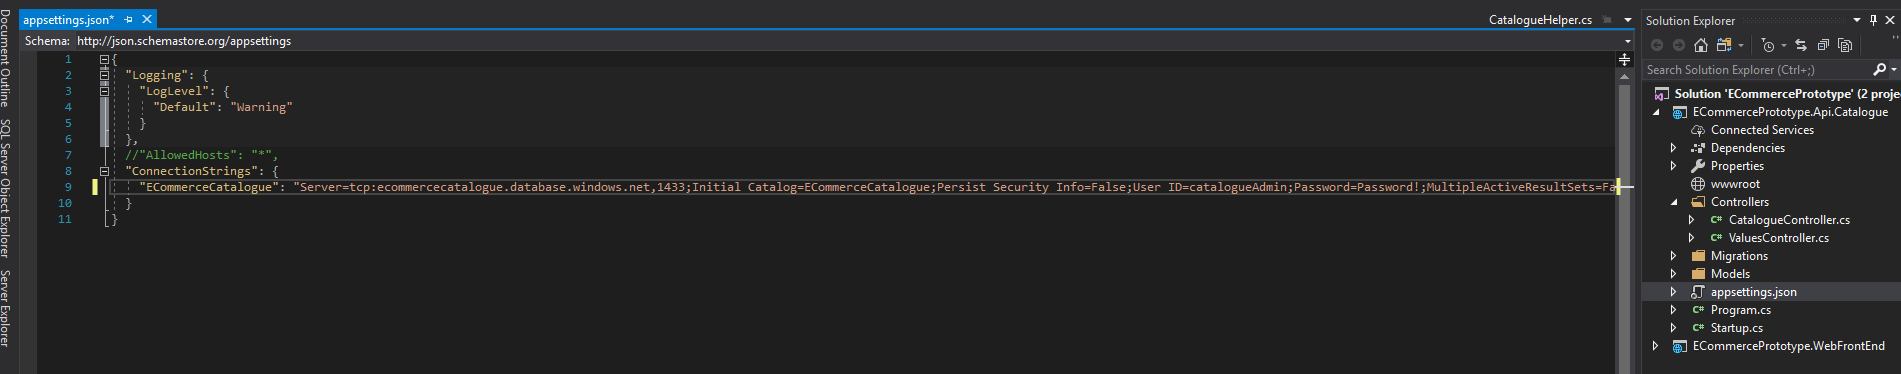
\includegraphics[height=5cm, width=15cm]{/DevelopmentPics/VSConnectionStringCatalogueMSImage}
\end{figure}

Using the Microsoft.Docs website, specifically the Entity Framework (EF) section, is very useful to gain an understanding, with example tutorials provided on how to use this feature for Database Manipulation \cite{EFMicrosoft}, \cite{EFMicrosoftQuickStart}. Also, an interesting blog on the c-sharpcorner website on this \cite{EFCSharpCorner}. And this blog (INSERT CITATION)

After reading over these sites. The project was started. Developing the Catalogue API first. Connection string and Entity framework were first to be created and inserted. Creating a DBContext class for the system to interact with the Catalogue database. This class inherits from the DBContext class that enables a session created with the databases, getting the connection string through the Appsettings.JSON file, and allows for querying and saving entities to the database. 

The Catalogue class was created using the system.ComponentModel.DataAnnotations.Schema to enable the properties to be used to create columns within the created table, within the CatalogueDB, that would store all catalogue item records. This was done by using Entity frameworks migration function to create the table based on the structure of the class and then updating the database with this migration. This was done successfully. Proving the system was connected to this database, through the Azure server, successfully. Of note, the Property storing the location of the picture for the item was not created at this point. It was done later.
 
Based on research (INSERT CITATION) it was deemed necessary to provide an interface that would provide the methods needed, for this microservice, to query the database. Specifically Getall() and Get(int id) methods. From here, the CatalogueManager class was created, that inherits from this interface. To provide implementation of these methods. The CatalogueManager class creates a read-only only object of the CatalogueDbContext that it uses to perform the methods upon. Returning the required entities - either a full list of all Catalogue Items or a single item based on its id in the database. 

To enable this database connection to be used repeatedly, the DBContext, Data Repository interface and data manager class needed dependency injection by adding them as services to the ConfigurstionServices method of startup class \cite{DependInjectMicrosoft}. BY setting the data repository \& catalogue manager as both scoped and transient, ensures each interaction with the database is created each time its requested and only once per request. Preventing duplication of requests within the one request.
\begin{figure}[h]
	\caption{Visual Studio Dependency Injection for the Catalogue Microservice}
	\label{fig:VSDICataMs}
	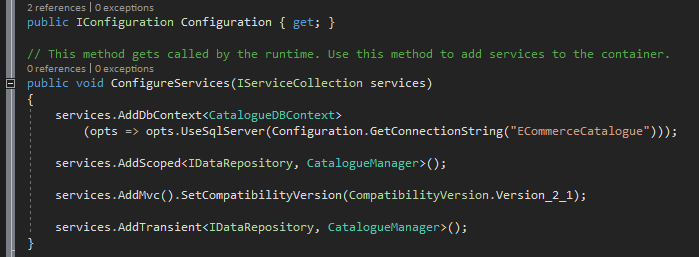
\includegraphics[height=6.5cm, width=15cm]{/DevelopmentPics/VSDICataMSImage}
\end{figure}

The final part of the Catalogue microservice to complete was the API Controller. This controller would be controlling how the database is interacted with, using HTTP Verbs, to expose what the front-end website can consume from this microservice. As the controller will be using a read-only object of the IDataRepository class, the only verbs being exposed will be Getall() and get() a single catalogue item by its id in the database.
\begin{figure}[h]
	\caption{Visual Studio API Controller for Catalogue Microservice}
	\label{fig:VSAPiCataMs}
	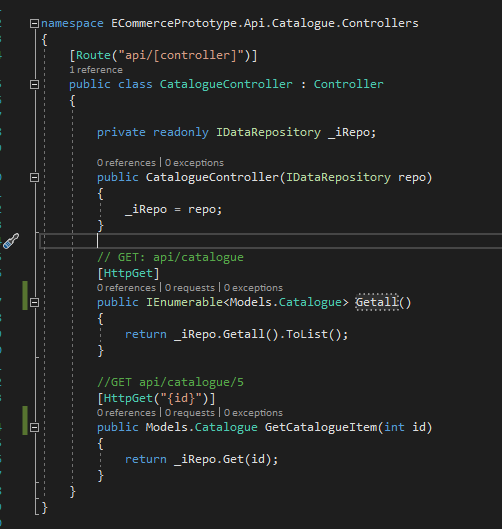
\includegraphics[height=12cm, width=11cm]{/DevelopmentPics/VSCataAPIController}
\end{figure}
Microsoft SQL server management system was used to connect to the database, trough its server, to insert several records to display on the website. After the inserts created, they were checked within the Azure portal dashboard to see they were present.

The Microservice was also run, as an API on the localhost, to display all the records created. And that a single record can be viewed by passing in an id to the URL.

(INSERT PICS??)

\subsubsection{Basket Microservice}

NOTE: All API's will be created using the same design of a DBContext, IDataRepository and Manager interfaces/classes. Only differences being naming convention and CRUD implementation. Which will be identified for each API.
\subsubsection{Prototype Development with a single centralised database}
\subsubsection{Front-End website development}
The website will be developed using the MVC architecture pattern. The Views applicable to each Microservice will be separated, as the standard when developing web applications using .NET Core, using folders. Each folder named after the corresponding controller that controls each group of Views.
To emphasise the use of Agile throughout the development cycle, the website will be developed upon after each Microservice has been successfully implemented. The different sections being developed are discussed:
\paragraph{Displaying Catalogue Items}
This section of the prototype was created with the MVC template provided by Microsoft as the basis. The implemented code was replaced with the required code for views and controllers.
Firstly, the models needed were created. A copy of the catalogue class from the Catalogue Microservice was created, as this would be needed to create an object of each record to be stored in another class, CatalogueItemRepository, that would be used by the View to display each catalogue Item, as per the initial class diagram design.

For the consumption of the API by the controller, a Catalogue API class was created, this would use the HTTPClient class to create a connection to the URL address of the Catalogue Microservice API. Adding a header to information sent in JSON format. This Class implemented its method through the Interface, ICatalogueAPI, that it inherits form. To allow for features to be added in the future, also to Inject Dependency, in the same fashion as data repository class of the Catalogue Microservice. Without this, it would be impossible for calls, after the initial call, to be conducted as the first call would still be using the connection. 

The controller for the views representing the catalogue Microservice 
	\pagebreak
	\subsection{Testing}
	\pagebreak
	\subsection{Evaluation}

	
	\pagebreak
	\section{Chapter 5: Conclusion/Evaluation}
	\pagebreak
	\bibliography{Bibliography}
	\bibliographystyle{plain}
	\pagebreak
	%example of References. See https://en.wikibooks.org/wiki/LaTeX/Bibliography_Management
	%might be good to use a separate document for these so your main work is not one really long text file. 
	
	%you can crate this on a extra Tex document just like the title or any other part of the document.
	\newpage
	\begin{appendices}
		\section{Project Initiation Document}
		%insert IPO
		
		\begin{subappendices}
			\subsection{Example sub appendices}
			...
		\end{subappendices}
		
		\section{Second Formal Review Output}
		Insert a copy of the project review form you were given at the end of the review by the second marker
		
		\section{Diary Sheets (or other project management evidence)}
		Insert diary sheets here together with any project management plan you have
		
		\section{Appendix 4 and following}
		insert content here and for each of the other appendices, the title may be just on a page by itself, the pages of the appendices are not numbered, unless an included document such as a user manual or design document is itself pager numbered.
	\end{appendices}
	
\end{document}